%
% File acl2018.tex
%
%% Based on the style files for ACL-2017, with some changes, which were, in turn,
%% Based on the style files for ACL-2015, with some improvements
%%  taken from the NAACL-2016 style
%% Based on the style files for ACL-2014, which were, in turn,
%% based on ACL-2013, ACL-2012, ACL-2011, ACL-2010, ACL-IJCNLP-2009,
%% EACL-2009, IJCNLP-2008...
%% Based on the style files for EACL 2006 by
%%e.agirre@ehu.es or Sergi.Balari@uab.es
%% and that of ACL 08 by Joakim Nivre and Noah Smith

\documentclass[11pt,a4paper]{article}
\usepackage[hyperref]{acl2018}
\usepackage{times}
\usepackage{latexsym}
\usepackage{hyperref}
\usepackage{listings}
\usepackage{graphicx}

\usepackage{url}

\aclfinalcopy % Uncomment this line for the final submission
%\def\aclpaperid{***} %  Enter the acl Paper ID here

\setlength\titlebox{5cm}
% You can expand the titlebox if you need extra space
% to show all the authors. Please do not make the titlebox
% smaller than 5cm (the original size); we will check this
% in the camera-ready version and ask you to change it back.

\newcommand\BibTeX{B{\sc ib}\TeX}

\title{CMSC 723 - Final Project Report}


\author{Dennis Cai, John Kanu, Allen Leis, Zhouchen Luo, Lingze Zhang \\
  University of Maryland \\ College Park, MD \\
  %\{dcai, jkanu, aleis, zluo, lzhang\}@umd.edu \\
}
\date{}

\begin{document}
\maketitle
\begin{abstract}
  We introduce a number research initiatives in support of developing a better question answering system for the \textsc{QANTA} competition.  For feature engineering we present keyword analysis, question categorization, and \textsc{TF/IDF} by paragraph.  We also develop a small ensemble model using \textsc{TF/IDF} and a Deep Averaging Network in order to obtain results in the downstream task of question answering.
\end{abstract}


\section{Introduction}

In support of developing a system for Question Answering is Not a Trivial Activity (\textsc{QANTA}) we have undertaken a number of research projects in order to produce a competitive system.  The projects described in this paper generally fall under the strategies of feature engineering and model enhancement.

The remainder of this document lists our research activities including motivation (why this is a good idea), methodology (what we did), and experimental results (whether our technique worked).  Due to space limitations we have omitted other research areas such as our \textsc{TF/IDF} error analysis, LSTM, and others.

Much of our research can be found in the following Github repositories:

\begin{itemize}
  \itemsep0em
  \small
  \item \url{https://github.com/looselycoupled/qanta-codalab}
\end{itemize}

\begin{figure*}[t]
  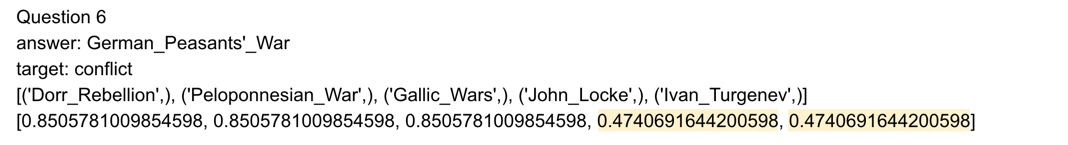
\includegraphics[width=\textwidth]{assets/question-6.png}
  \caption{Keyword analysis of candidate answers}
  \label{fig:question6}
\end{figure*}


\section{\textsc{TF/IDF} Hyperparameter Search}

\subsection{Motivation}
Our first endeavor was to try and improve upon the existing \textsc{QANTA} baseline by performing a hyperparameter search in order to maximize accuracy of the system and develop a new baseline for comparison.

\subsection{Methodology}
Hyperparameter searches can be notoriously time and resource consuming.  As an example, the TfidfVectorizer from Python’s scikit learn library contains at least fourteen different input parameters that can have a significant effect on final accuracy.  With each parameter having a minimum of two values to evaluate, this leads to 2\textsuperscript{14} possible combinations to evaluate.  To reduce this number we focused on only 8 hyperparameters and took a two pronged approach.

First we tested with default values and changed only a single value at a time using a small set of possible values per parameter to identify high impact parameters and targets.  We followed up with a combinatorial approach that led to only 180 permutations to test.  Note that one of our hyperparameters was a flag for whether or not to include stemming within the preprocessing portion of the vectorizer.

\subsection{Experimental Results}
Our experiments concluded that the best results could be found with the following inputs:

\begin{verbatim}
{
 `lowercase': True,
 `max_df': > .75,
 `max_features': None,
 `min_df': 2,
 `ngram_range': [1, 2],
 `norm': 'l2',
 `stop_words': `english',
 `stemming': False
}
\end{verbatim}

Training with these values on \textit{quanta.train.2018.04.18.json} and evaluating on \textit{quanta.test.2018.04.18.json} provides an accuracy of .54 which is several percentage points above the default.

\section{Question Categorization}

\subsection{Motivation}
Attempt to rule out potential answers by comparing category of the question to category of the predicted answers.

\subsection{Methodology}
First, we extracted the data from the \textsc{QANTA} JSON files to get a master list of high level categories (11) and subcategories (102).  Then we developed a Deep Averaging Network (\textsc{DAN}) for classification and trained it on the \textsc{QANTA} training data using undersampling to deal with class imbalance.

\subsection{Experimental Results}
We were able to achieve an accuracy of 83\% when predicting question category.  Unfortunately, this research proved unhelpful as multiple guesses returned by our models tend to all come from the same category.


\section{Keyword Analysis}

\subsection{Motivation}
In examining question text, we wanted to exploit sentence structure by making use of the subject of the word \textit{this} or \textit{these} as in \textit{this author} which we refer to as the target keyword.  By using this keyword, we hope to eliminate potential answers that do not appear to refer to the target, and by extension the correct answer.

\subsection{Methodology}
At a high level, we use facts about our potential answers and compare the appropriate word embedding to the target keyword using cosine similarity. Our facts come from the \textsc{YAGO} \textit{yagoSimpleTypes} dataset provided by the Max Planck Institutes which is built from the  Wikipedia, WordNet and GeoNames datasets .  This data captures semantic information in the form of \textsc{RDF} triples such as ``subject'', ``predicate'', ``object''.

\subsection{Experimental Results}

Experimental results are initially very promising as our code is able to correctly identify answers that best match the target keyword.  As an example from the test dataset, one target keyword is \textit{conflict} for the ultimate answer of \textit{German\_Peasants\_War} as shown in \autoref{fig:question6}.

The system correctly notes the high similarity for the first three answers while providing lower similarity scores for the names of individuals.  However, note that none of these answers are actually correct which leads us to the reasons why this methodology was ultimately left out of the final answering system.

In general, the methodology works well but is inconsistent enough that we do not trust it to overrule the model's first choice.  A number of failure modes are possible such as:

\begin{itemize}
  \itemsep0em
  \item  Correct answer is not in any potential answer
  \item  Null results from \textsc{\textsc{YAGO}} dataset or when parsing for the \textsc{NNS}
  \item  The correct answer may not have the highest similarity due to word choice in the \textsc{\textsc{YAGO}} data
  \item  Irrelevance if all answers are of the same underlying type (such as the name of a play)
 \end{itemize}


\section{Deep Averaging Network Answer Model}

\subsection{Motivation}
For our Deep Averaging Network (\textsc{DAN}) we were motivated to explore alternative models for direct question answering.

\subsection{Methodology}
We took two general approaches to model development with our \textsc{DAN}.  First, we went with a relatively basic approach with 3000 hidden nodes and 26,878 output nodes for classification using the \textsc{QANTA} training data.  An alternate version was also constructed with 7000 hidden nodes to try to improve overall classification accuracy.  After disappointing results with our initial \textsc{DAN}, we returned to the academic literature and settled upon ``Deep Unordered Composition Rivals Syntactic Methods for Text Classification'' (Iyyer et al).

\lstset{frame=tb,
  language=Python,
  aboveskip=3mm,
  belowskip=3mm,
  showstringspaces=false,
  columns=flexible,
  basicstyle={\small\ttfamily},
  numbers=none,
  numberstyle=\tiny\color{gray},
  breaklines=true,
  breakatwhitespace=true,
  tabsize=2
}
\begin{lstlisting}[caption={\textsc{DAN} Architecture},captionpos=b,label={lst:dan}]
DanModel(
  (embeddings): Embedding(3000000, 300, padding_idx=0)
  (encoder): DanEncoder(
    (encoder): Sequential(
      (0): Linear(in_features=300, out_features=14000, bias=True)
      (1): BatchNorm1d(14000, eps=1e-05, momentum=0.1)
      (2): ELU(alpha=1.0)
      (3): Dropout(p=0.05)
    )
  )
  (dropout): Dropout(p=0.05)
  (classifier): Sequential(
    (0): Linear(in_features=14000, out_features=26878, bias=True)
    (1): BatchNorm1d(26878, eps=1e-05, momentum=0.1)
    (2): Dropout(p=0.05)
  )
)
\end{lstlisting}

Upon reviewing Iyyer's research and related work online and in the ``Pinafore/qb'' repository, we set out to create a more advanced \textsc{DAN} based on designs we were encountering for the same downstream tasks (see \autoref{lst:dan}).

\subsection{Experimental Results}
Our initial \textsc{DAN} architectures provided poor prediction accuracy, took a long time to train (29 hours), and did not appear to outperform the baseline \textsc{TF/IDF} system. Meanwhile, our improved \textsc{DAN} model completed training after 50 epochs (3 hours) and attained a final accuracy of 0.38 on the test set (Figure 5). In the \texttt{docker-compose run eval} downstream task we were able to attain an ``end\_acc'' of 0.42193140794223827, an ``expected\_wins'' of  0.12742574327151907, and an ``expected\_wins\_optimal'' score of  0.5845992400723761.  Note that ``first\_acc'' was always zero for all downstream testing with the \textsc{DAN} models.


\section{Ensemble Answer Model}

\subsection{Motivation}
For our ensemble method, we were looking to leverage multiple models to improve overall accuracy.

\subsection{Methodology}

\begin{figure}[ht]
  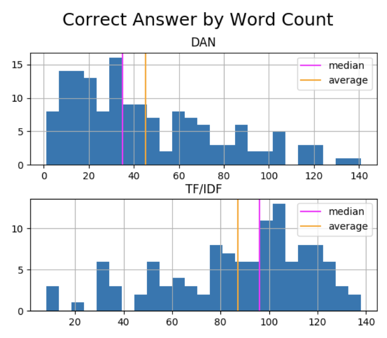
\includegraphics[width=\columnwidth]{assets/answer-word-count.png}
  \caption{Answer By Word Count}
  \label{fig:ans_by_count}
\end{figure}

We first chose to evaluate the accuracy of our models over time to focus on the downstream task of the \textsc{QANTA} evaluation.  We sampled 200 questions and fed them into the models word by word, checking the accuracy of the top guesses along the way (\autoref{fig:ans_by_count}).  Our evaluation shows that the \textsc{DAN} finds the correct answer on average much sooner than \textsc{TF/IDF} with a mean of 45 words and a median of 35  words compared to a mean of of 87 and a median of 96 words.  Using this information, we formulated several strategies for choosing between the two models and compared their results.

\subsection{Experimental Results}

\begin{table}[htb]
\tiny
\begin{tabular}{|l|l|l|}
\hline
Evaluation              & Docker Eval Results & CodaLab Macro Results \\ \hline
first\_acc              & 0.0                 & 0.049707602339181284  \\ \hline
end\_acc                & 0.42193140794223827 & 0.3847465886939571    \\ \hline
expected\_wins          & 0.15221777278922483 & 0.08030731291105844   \\ \hline
expected\_wins\_optimal & 0.5845992400723761  & 0.48729618157593796   \\ \hline
\end{tabular}
\caption{Ensemble Model Evaluation Results}
\label{table:results}
\end{table}

In our best performing approach, we allow the \textsc{TF/IDF} to buzz in for the first 50 words based on the baseline guessing logic.  After 50 words, we immediately buzz in to beat the opponent to the buzzer and submit the  top answer from the \textsc{DAN} model.  Our local \texttt{docker-compose run eval} scores and CodaLab macro scores are listed in \autoref{table:results}.

Other  methods were explored (such as letting both models guess at any time) but offer less expected wins with other statistics remaining roughly the same. Our intuition is that the by forcing a guess at 50 words, we are able to beat the opponent to the buzzer whether the model is confident or not.  For future work we would like to build a classifier to help choose the model to use based on question content, logits returned, etc.


\section{\textsc{TF/IDF} By Paragraph Answer Model}

\subsection{Motivation}
To explore alternative approaches and at the suggestion of the professor, we set out to research the accuracy of using raw wikipedia text and feed it into our \textsc{TF/IDF} model.  Our novel approach would be to submit each paragraph from an article as a separate document.  The intuition is that single paragraphs are more dense with information and should score a higher similarity when guessing.

\subsection{Methodology}
We began by using the wikiextractor tool (recommended by the TAs) on our 12GB dump of Wikipedia articles to convert them into JSON files.  Using this data we found the correct article titles to match the \textsc{QANTA} datasets using the MediaWiki API at \url{https://en.wikipedia.org/w/api.php}.  Then we split article text according to line breaks, however we chose to combine paragraphs under 300 characters with the subsequent paragraph as we felt these very small paragraphs lacked enough information after reviewing them.

We create our \textsc{TF/IDF} model and fit it with the paragraph data, with multiple paragraphs (now separate documents) corresponding to the same Wikipedia page title.  The sklearn TfidfVectorizer is used with ngram\_range=(1, 1), min\_df=2, max\_df=.75 as the hyperparameters.  ngram\_range was limited to unigrams for memory and processing considerations.

\subsection{Experimental Results}
Upon examination of the processed data, we found that number of paragraphs per article is generally low but has an extremely long tail.  Using our methodology we identified 15,922,351 paragraphs over 3,354,819 articles.   We found that that articles have an average of 4.75 paragraphs with a standard deviation of 7.51, a median of 2.0, and a maximum of 489.0 (see \autoref{fig:paracount}).  1,128,471 articles (one third of the corpus) contains only a single paragraph.

\begin{figure}[ht]
  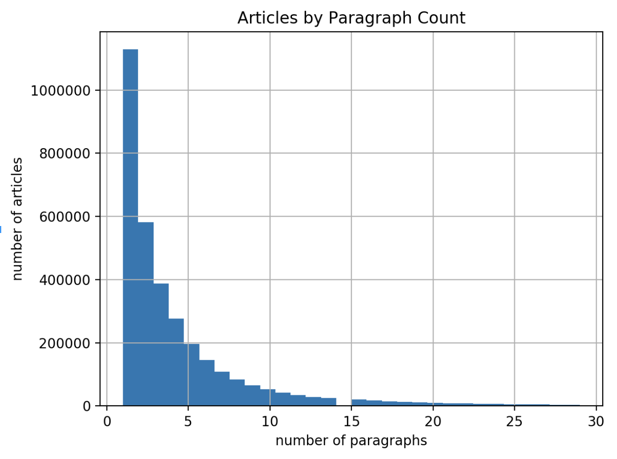
\includegraphics[width=\columnwidth]{assets/articles-by-para-count.png}
  \caption{Articles By Paragraph Count}
  \label{fig:paracount}
\end{figure}

Using the original 12GB dataset to load into \textsc{TF/IDF}, we were able to get an accuracy of 0.04 on the first 500 questions in the test dataset with 21 correct responses.  Because of the initial poor results, and time constraints for these experiments, we did not process the full test dataset but spent our time analyzing the failure modes of the model.

To look at one failure example (which is representative of the data), let’s take the first item from the test dataset in which the answer is \textit{Francis\_Bacon} and the word \textit{ambition} appears three times.

The model produces the following answers: Ambition\_(charity), London\_Councils, Novum\_Organum, Novum\_Organum, Grit\_(personality\_trait).  The \textit{Ambition\_(charity)} paragraph contains the word \textit{ambition} eleven times.  The \textit{London\_Councils} paragraph contains the bigram \textit{Capital Ambition} five times.  The two \textit{Novum\_Organum} paragraphs have the bigram \textit{Novum Organum} (a philosophical work by Francis Bacon which appears in the question) four and two times respectively but keep in mind these tokens have a low document frequency.  And finally the paragraph about \textit{Grit\_(personality\_trait)} contains the word \textit{ambition} three times.

The model is correctly finding similar paragraphs according to the \textsc{TF/IDF} algorithm but because there are so many documents it becomes easy to stumble into the wrong answer purely on word frequency.  Also, pages chosen for competition are likely to be less obscure and so will have many related articles with their own paragraphs for \textsc{TF/IDF} to choose instead of the correct page (such as the Novum\_Organum example).  Finally, almost 2/3 of the articles contain three or less paragraphs so splitting them up may not be adding much value.  A 500 question sample of test dataset responses including model guesses and corresponding article paragraphs can be found for further review at \url{https://goo.gl/HMDGMY}.

For further research we would like to start with examining the relationship of articles with many paragraphs vs those with few.  Do articles with more paragraphs appear more often in results because there are more “documents” in the model pointing to the same Wikipedia article?  We would also like to explore bigrams and find a way to split articles into sections rather than paragraph.

Finally, we have concerns about the practicality of this approach in a competition as the python process used over 18 GB of RAM to hold this model and python would not save it do disk (using pickle) as it was over 4GB.  Training time is over an hour on an EC2 p2.xlarge (4 CPU, 60GB RAM) and so it would be time consuming to train/fit at competition.




\end{document}
